\subsection*{Context of the internship}

As part of the \href{http://informatique.ens-lyon.fr/en/academic-programs/master/m1}{first year of Master} at the
\href{http://www.ens-lyon.fr/en/}{École Normale Supérieure de Lyon},
I was able to do a 12 weeks research internship in a laboratory.

My research for an internship in Quantum Algorithmic have brought me to
the \href{https://www.lu.lv/en/studies/faculties/faculty-of-computing/}{Faculty of Computing}
at the \href{https://www.lu.lv/}{University of Latvia}
and my supervisor \href{http://home.lu.lv/~ambainis/}{Andris Ambainis}. My research also
brings me to discuss with \href{https://kpfu.ru/Kamil.Hadiev?p_lang=2}{Kamil Khadiev}
from \href{https://eng.kpfu.ru/}{Kazan Federal University} who has become my co-supervisor.
We have discussed by email to find an interesting subject of research on which I have
liked to work on. I thank them for their help, their supervision and the time they have
given to me during this 12 weeks.

During the internship, I have been integrated to the life of the
\href{https://quantum.lu.lv/}{Center for Quantum Computing Science}.
I thanks members of the team for the great discussions we had after
the seminar.

I also want to thank \href{https://perso.ens-lyon.fr/omar.fawzi/}{Omar Fawzi} for
having introduced me to quantum computing and its fascinating possibilities.

The team's research area is quantum algorithms and complexity theory. More precisely,
the team works on establishing new quantum algorithm with better complexity and proving
new lower bound to the quantum complexity for many different type of problem belonging
from graph theory to cryptography passing by language  recognition theory. My work on
the recognition of restricted Dyck words integrate itself great in the team work as it
has already been studied by the team few years ago \cite{art:2DGrid} and further by
Kamil Khadiev \cite{DBLP:conf/uc/KhadievK21}.

My internship, named "Complexity of recognizing Dyck language with a
quantum computer", as for goal to reduce the gap between the lower and the upper bound for
a quantum query algorithm that recognizes Dyck words of bounded height. The best
lower and upper bound are describe in \cite{art:2DGrid} by Andris Ambainis team.

In the end of the introduction the field of research will be presented more precisely.
After that, technical preliminaries, which are useful to understand the
current and the new results, ill be detailed. Finally, the last section presents the
new results on the problem and the failures.

\subsection{History of quantum computing}

The history of quantum computing has started in 1980 when Paul Benioff, an american physicist,
proposed a quantum mechanical model of the Turing machine \cite{art:paulbenioff}.
This machine use some properties
of the matter that has been discovered by quantum physicist. After that, some computer
scientists suggested that the quantum model of turing machine may be more expressive that the
classical model. Few years after, the first bricks of the quantum circuit have been introduced
by Richard Feymann \cite{art:feymann}. The first quantum computers have started to arrived middle
of 1990s. During the last 20 years, the founds given to the creation of the first quantum computer
have skyrocketed, as the number of start-up and company dedicated to it. This emulation has made
from the quantum computer
field one of the most active field of research today. On the algorithmic side, the first
astonishing result is the algorithm designed by Peter Shor (1994) \cite{art:shor}. The
algorithm improves a lot the complexity of factorizing integers, enough to break our
cryptographic protocols when quantum computer will be powerful enough. Since 1994, the
quantum algorithm area has evolved almost independently from the quantum computers and
has developed many beautiful theories and interesting results. But how does a quantum
circuit works?

\subsection{The quantum circuit, and quantum query model and complexity}

In classical computer science, the piece of information is represented by using
0 and 1. This two states can be easily obtained using electricity with 0 equal to 0V
and 1 equal 5V. It is easy to propagate electricity through wires and to stock its
level into capacitor. Moreover a little piece of hardware, named transitor, has allow to do some
computations using logical gates which when include in a complex machine create our
so-called "computers".

In quantum computer, the story isn't so different. First, the 0 and 1 are
now represented using particles like electrons or photons. For example,
an electron with a spin of $+\frac{1}{2}$ (note \ket{1}) represents a 1 and
an other one with a spin of $-\frac{1}{2}$ (note \ket{0}) represents a 0.
But the use of particles is motivated by their properties and mainly by
a quantum property called superposition. A quantum state is not only \ket{0}
or \ket{1}, but can be $\lambda_0 \ket{0} + \lambda_1 \ket{1}$ for every
$\lambda_{0, 1} \in \mathbb{C}$ such that $\lambda_0+\lambda_1=1$ and a quantum
bit is now called a qubit. As before, the computations are done by gates, here
quantum gates which transform the quantum state of the qubit into another one.
At the end, to get the result of a computation, it is mandatory to measure the
state of the quantum system, which break the quantum superposition. A quantum
state of $n$ qubits can be represented with a length 1 vector in a $2^n$
dimensional space and a quantum gates by a linear unitary transformation
on a $2^n$ dimensional space. A transformation is said unitary if is preserved
the length.

\paragraph*{A quantum circuit} is a precise configuration of quantum gates
on a finite number of qubits. The following \autoref{fig:quantum_circuit_examle} represents the quantum
circuit that computes a uniform randomize on $\{0, 1\}^n$.

\begin{figure}[h!]
    \begin{minipage}{.30\textwidth}
        \centering
        $
            \Qcircuit @C=.8em @R=1em {
            \mbox{$n$ \textrm{entries}} &     &                              &     & \mbox{$n$\ \textrm{outputs}}    \\
            \lstick{\ket{0}} & \qw & \multigate{2}{H^{\otimes n}} & \qw & \meter & \cw\\
            \vdots & & \ghost{H^{\otimes n}} & \qw & \vdots &\\
            \lstick{\ket{0}}& \qw & \ghost{H^{\otimes n}} & \qw & \meter & \cw\\
            }$
    \end{minipage}
    \hfill
    \begin{minipage}{.65\textwidth}
        \textbf{Legend:}

        $ \bullet \
            \Qcircuit @C=1em @R=1em {
            & \qw & & \cw \\
            }$ are respectively a quantum wire and a classical wire.

        $\bullet \ \Qcircuit @C=.4em @R=.4em {
            & \gate{H^{\otimes n}} \\
            }$ is the Hadamard's gates on each input qubit.

        $\bullet \ \Qcircuit @C=.4em @R=.4em {
            & \meter \\
            }$ is the measure of 1 qubit in the algorithm.
    \end{minipage}
    \caption{A quantum circuit computing the uniform random on $\{0, 1\}^n$. }
    \label{fig:quantum_circuit_examle}
\end{figure}

\paragraph*{The quantum query circuit} is a quantum circuit used to
compute function with an entry space where $x=x_1 \ldots x_N$ belongs.
The black box model \cite{black_box_andris} of a quantum query circuit is composed of
an input state $\ket{\psi_ {start}}$ and a sequence
$U_0, Q, U_1, \ldots, Q, U_T$ of linear unitary transformations such that $\ket{\psi_{start}}$ and all $U_i$
do not depend on entry $x$ unlike the $Q_i$ which depend on $x$. The quantum state
$\ket{\psi_ {start}}$ belong to a $d$-dimensional space generated
by $\ket{1}, \ket{2},\ldots, \ket{d}$.  To define $Q$, the basis vectors first need to
be renamed from $\ket{1},\ldots, \ket{d}$ to $\ket{i, j}$ with
$i \in \llbracket 0, N\rrbracket$ and $j \in \llbracket1, d_i \rrbracket$ for some
$d_i$ such that  $d_1 + d_2 + \ldots + d_N = d$. Next, $Q$ is define such that

\[Q(\ket{i, j}) := \left\{
    \begin{array}{ll}
        \ket{0, j}  & \textrm{if\ } i = 0                           \\
        \ket{i, j}  & \textrm{if\ } i > 0 \ \textrm{and\ } x_i = 0  \\
        -\ket{i, j} & \textrm{if\ } i > 0 \ \textrm{and\ } x_i = 1.
    \end{array}
    \right.  \]

The gates $Q$ are doing the queries to input $x$ by flipping some of the vectors.
Finally, to get the output of the quantum query algorithm it is necessary to
measure the output. A quantum query algorithm can the summarized with the following
quantum circuit.

\begin{figure}[h!]
    \centering
    $
        \Qcircuit @C=.8em @R=1em {
        \lstick{\vdots} & \qw & \multigate{2}{U_0}  & \multigate{2}{Q} & \multigate{2}{U_1} & \qw &  & &  \multigate{2}{Q} & \multigate{2}{U_T}&\multigate{2}{\metersymbol{.2}} & \cw\\
        &\lstick{\ket{\psi_{start}}} qw & \ghost{U_0} & \ghost{Q} & \ghost{U_1} & \qw & \cdots & & \ghost{Q} & \ghost{U_T} & \ghost{\metersymbol{.2}}& \cw\\
        \lstick{\vdots}& \qw & \ghost{U_0} & \ghost{Q}  & \ghost{U_1} & \qw & & &\ghost{Q} &\ghost{U_T}&\ghost{\metersymbol{.2}}& \cw \\
        }$
    \caption{Structure of a quantum query algorithm.}
    \label{fig:quantum_query_algorithm_structure}
\end{figure}

\paragraph*{The quantum query complexity} of an algorithm corresponds to the number of calls to the $Q$ gate. Often, this number of calls
is depending on the size of the entry. The quantum query complexity of a problem corresponds to the higher bound for which it is
certain there is no quantum query algorithm with a greater quantum query complexity solving the problem.

\subsection{Dyck Languages of height $k$}

First, the Dyck Language corresponds to the set of correct and balanced word  of parenthesis.
The Dyck language is a context free language as it can easily be recognized using a context
free grammar. The work done by Andris Ambainis' team \cite{art:2DGrid} focus on a restriction
Dyck language with fixed height $k$. More precisely, a Dyck word has a height of $k$ if, in every
of its prefix, the difference between the number of opening and closing parenthesis does not
exceeds $k$. These restricted Dyck languages are called \Dyck{k,n} and are interesting because
they belong to the already well studied class of star free languages (Detail in \autoref{ssec:starfree}).

\begin{figure}[h!]
    \centering
    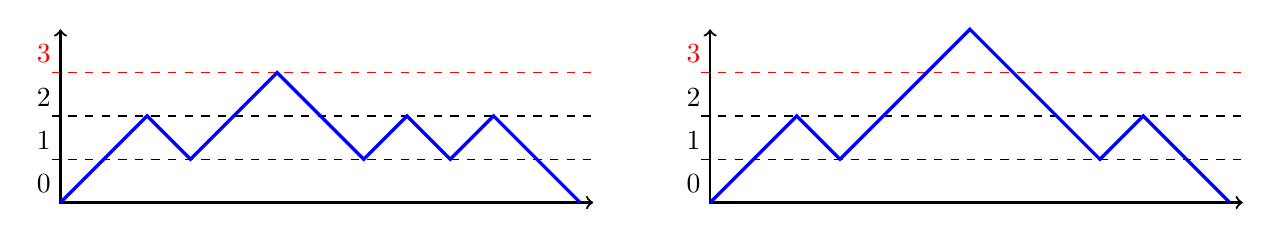
\begin{tikzpicture}[scale=.55]
        \draw[<->, thick] (0, 4) -- (0, 0)  -- (12.3, 0);
        \draw[dashed] (-.2, 1) -- (12.3, 1);
        \draw[dashed] (-.2, 2) -- (12.3, 2);
        \draw[dashed, red] (-.2, 3) -- (12.3, 3);
        \draw[blue, very thick] (0, 0) -- (2, 2) -- (3, 1) -- (5, 3) -- (7, 1) -- (8, 2) -- (9, 1) -- (10, 2) -- (12, 0);
        \draw (0, 0) node[above left] {0};
        \draw (0, 1) node[above left] {1};
        \draw (0, 2) node[above left] {2};
        \draw[red] (0, 3) node[above left] {3};

        \draw[<->, thick] (15+0, 4) -- (15+0, 0)  -- (15+12.3, 0);
        \draw[dashed] (15+-.2, 1) -- (15+12.3, 1);
        \draw[dashed] (15+-.2, 2) -- (15+12.3, 2);
        \draw[dashed, red] (15+-.2, 3) -- (15+12.3, 3);
        \draw[blue, very thick] (15+0, 0) -- (15+2, 2) -- (15+3, 1) -- (15+6, 4) -- (15+9, 1) -- (15+10, 2) -- (15+12, 0);
        \draw (15+0, 0) node[above left] {0};
        \draw (15+0, 1) node[above left] {1};
        \draw (15+0, 2) node[above left] {2};
        \draw[red] (15+0, 3) node[above left] {3};
    \end{tikzpicture}
    \caption{\textbf{On the left}, a valid Dyck word of height 3. \textbf{On the right}, an invalid Dyck word of height 3.}
    \label{fig:dyck_word}
\end{figure}

\subsection{State of the art}
This state of the art will not be to precise as the understanding of the
bibliography has taken almost the first half the internship and will be
more detailed in the \autoref{sec:preli}. First, few years ago Aaronson,
Grier and Schaeffer \cite[2019]{trichotomy_not_andris} worked on quantum complexity
of recognizing regular languages as they can model a lot of tasks. They
concluded that there are 3 different cases depending of the language:
\begin{itemize}
    \item $O(1)$ if it is sufficient to read constant number of letters at the beginning and the end.
    \item $\tilde{\Theta}(\sqrt{n})$ if a Grover's search is the best way to recognize the language.
    \item $\Theta(n)$ if recognizing the language is the same as counting modulo some value that can
          be computed with $O(n)$.
\end{itemize}
Further more, it is proved that being in the second classes is equivalent to
being a star free language. Andris ambainis' team decided to work on \Dyck{k, n} as this
language is a beautiful example of star free languages. In \cite[2020]{art:2DGrid},
the team focus on the power of the logarithm in $\tilde{\Theta}\left(\sqrt{n}\right)$.
They first proved by reduction that the quantum query complexity of \Dyck{k, n}
called $Q\left(\Dyck{k, n}\right)$ is in $\Omega\left(c^k\sqrt{n}\right)$ where $c$ is
a constant greater than 1 and after gave an algorithm for \Dyck{k, n} with a quantum
query complexity of $O\left(\sqrt{n}(\log(n))^{0.5k}\right)$. Since then, no better
lower bound or algorithm have been found.

\subsection{Goals of the internship}
The problem on the quantum query complexity of \Dyck{k,n} is still open, my internship
has for goal to reduce the gap between the lower bound and the best known algorithm.
The researches have been organized on two main axes:
\begin{itemize}
    \item \textbf{Increasing the lower bound.} To do this, It is necessary to understand the bibliography
          on the adversary method in order to try to find a new adversary with better property.
    \item \textbf{Lowering the upper bound.} It is sufficient to find new algorithms
          with a quantum query complexity better than  the previous best known algorithm's one.
\end{itemize}
Finally, the overall goal would be to made the two bounds match in order to get the exact quantum
query complexity of \Dyck{k,n}. Finally, the problem could also be reformulated for multi-brackets word
as done by Kamil Khadiev in \cite{DBLP:conf/uc/KhadievK21}.

\subsection{Results}

{\color{red} \Huge TODO}